%%%%%%%%%%%%%%%%%%%%%%%%%%%%%%%%%%%%%%%%%
% Oliver Lemon made minor edits (jan 2015)  to : 
% Masters/Doctoral Thesis 
% LaTeX Template
% Version 1.43 (17/5/14)
%
% This template has been downloaded from:
% http://www.LaTeXTemplates.com
%
% Original authors:
% Steven Gunn 
% http://users.ecs.soton.ac.uk/srg/softwaretools/document/templates/
% and
% Sunil Patel
% http://www.sunilpatel.co.uk/thesis-template/
%
% License:
% CC BY-NC-SA 3.0 (http://creativecommons.org/licenses/by-nc-sa/3.0/)
%
% Note:
% Make sure to edit document variables in the Thesis.cls file
%
%%%%%%%%%%%%%%%%%%%%%%%%%%%%%%%%%%%%%%%%%

%----------------------------------------------------------------------------------------
%	PACKAGES AND OTHER DOCUMENT CONFIGURATIONS
%----------------------------------------------------------------------------------------

\documentclass[11pt, oneside]{Thesis} % The default font size and one-sided printing (no margin offsets)

\graphicspath{{media/}} % Specifies the directory where pictures are stored

\usepackage[square, comma, sort&compress]{natbib} % Use the natbib reference package - read up on this to edit the reference style; if you want text (e.g. Smith et al., 2012) for the in-text references (instead of numbers), remove 'numbers' 
\hypersetup{urlcolor=blue, colorlinks=true} % Colors hyperlinks in blue - change to black if annoying

\usepackage{float}

\usepackage{longtable}
\usepackage[toc, acronym]{glossaries}

\newacronym{ml}{ML}{Machine Learning}
\newacronym{gd}{GD}{Gradient Descent}
\newacronym{bgd}{BGD}{Batch Gradient Descent}
\newacronym{rbfn}{RBFN}{Radial Basis Function Network}
\newacronym{mbgd}{MBGD}{Mini-Batch Gradient Descent}
\newacronym{sgd}{SGD}{Stochastic Gradient Descent}
\newacronym{dnn}{DNN}{Deep Neural Network}
\newacronym{mlp}{MLP}{Multi-Layer Perceptron}
\newacronym{rnn}{RNN}{Recurrent Neural Network}
\newacronym{cnn}{CNN}{Convolutional Neural Network}
\newacronym{relu}{ReLU}{Rectified Linear Unit}
\newacronym{cv}{CV}{Computer Vision}
\newacronym{fp}{FP}{Functional Programming}
\newacronym{ai}{AI}{Artificial Intelligence}
\newacronym{aiv}{AIV}{Artificial Intelligence Verification}
\newacronym{nn}{NN}{Neural Network}
\newacronym{mas}{MAS}{Multi-Agent System}
\newacronym{dl}{DL}{Deep Learning}
\newacronym{pl}{PL}{Programming Language}
\newacronym{pypl}{PYPL}{PopularitY of Programming Language Index}
\newacronym{smt}{SMT}{Satisfiability Modulo Theories}

\makeglossaries{}

\title{\ttitle} % BUT you should use use " \title{\ttitle} " here instead to define the thesis title ! 
% \ttitle is defined in the file Thesis.cls 

\begin{document}

\frontmatter % Use roman page numbering style (i, ii, iii, iv...) for the pre-content pages

\setstretch{1.3} % Line spacing of 1.3

% Define the page headers using the FancyHdr package and set up for one-sided printing
\fancyhead{} % Clears all page headers and footers
\rhead{\thepage} % Sets the right side header to show the page number
\lhead{} % Clears the left side page header

\pagestyle{fancy} % Finally, use the "fancy" page style to implement the FancyHdr headers

\newcommand{\HRule}{\rule{\linewidth}{0.5mm}} % New command to make the lines in the title page

% PDF meta-data
\hypersetup{pdftitle={\ttitle}}
\hypersetup{pdfsubject=\subjectname}
\hypersetup{pdfauthor=\authornames}
\hypersetup{pdfkeywords=\keywordnames}

%----------------------------------------------------------------------------------------
%	TITLE PAGE
%----------------------------------------------------------------------------------------

\begin{titlepage}
    \begin{center}

        \textsc{\LARGE \univname}\\[1.5cm] % University name
        \textsc{\Large Masters Thesis}\\[0.5cm] % Thesis type

        \HRule \\[0.4cm] % Horizontal line
        {\huge \bfseries \ttitle}\\[0.4cm] % Thesis title
        \HRule \\[1.5cm] % Horizontal line

        \begin{minipage}{0.4\textwidth}
            \begin{flushleft} \large
                \emph{Author:}\\
                \href{http://www.johnsmith.com}{\authornames} % Author name - remove the \href bracket to remove the link
            \end{flushleft}
        \end{minipage}
        \begin{minipage}{0.4\textwidth}
            \begin{flushright} \large
                \emph{Supervisor:} \\
                \href{http://www.jamessmith.com}{\supname} % Supervisor name - remove the \href bracket to remove the link  
            \end{flushright}
        \end{minipage}\\[3cm]

        \large \textit{A thesis submitted in fulfilment of the requirements\\ for the degree of \degreename}\\[0.3cm] % University requirement text
        \textit{in the}\\[0.4cm]
        %\groupname\\

        \deptnamefirst\\[0.4cm] % Research group name and department name

        % \&

        \deptnamesecond\\[0.4cm] % Research group name and department name

        \&

        \groupname\\[1.5cm]

        {\large \today}\\[1cm] % Date
        
\includegraphics[width=6cm]{./Figures/HWUlogo.jpg} % University/department logo - uncomment to place it

        \vfill
    \end{center}

\end{titlepage}

%----------------------------------------------------------------------------------------
%	DECLARATION PAGE
%	Your institution may give you a different text to place here
%----------------------------------------------------------------------------------------

\Declaration{

    \addtocontents{toc}{\vspace{1em}} % Add a gap in the Contents, for aesthetics

    I, \authornames, declare that this thesis titled, '\ttitle' and the work presented in it is my own. I confirm that this work submitted for assessment is my own and is
    expressed in my own words. Any uses made within it of the works of
    other authors in any form (e.g., ideas, equations, figures, text,
    tables, programs) are properly acknowledged at any point of their
    use. A list of the references employed is included.

    %\begin{itemize} 
    %\item[\tiny{$\blacksquare$}] This work was done wholly or mainly while in candidature for a research degree at this University.
    %\item[\tiny{$\blacksquare$}] Where any part of this thesis has previously been submitted for a degree or any other qualification at %this University or any other institution, this has been clearly stated.
    %\item[\tiny{$\blacksquare$}] Where I have consulted the published work of others, this is always clearly attributed.
    %\item[\tiny{$\blacksquare$}] Where I have quoted from the work of others, the source is always given. With the exception of such %quotations, this thesis is entirely my own work.
    %\item[\tiny{$\blacksquare$}] I have acknowledged all main sources of help.
    %\item[\tiny{$\blacksquare$}] Where the thesis is based on work done by myself jointly with others, I have made clear exactly what %was done by others and what I have contributed myself.\\
    %\end{itemize}
    \vspace{2cm} 
    Signed: Arran Dinsmore\\
    \rule[1em]{25em}{0.5pt} % This prints a line for the signature

    Date: \today\\
    \rule[1em]{25em}{0.5pt} % This prints a line to write the date
}

\clearpage % Start a new page

%----------------------------------------------------------------------------------------
%	QUOTATION PAGE
%----------------------------------------------------------------------------------------

\pagestyle{empty} % No headers or footers for the following pages

\null\vfill % Add some space to move the quote down the page a bit

\textit{``\textbf{Mistakes} are the portals of \textbf{discovery}."}

\begin{flushright}
    James Joyce
\end{flushright}

\vfill\vfill\vfill\vfill\vfill\vfill\null % Add some space at the bottom to position the quote just right

\clearpage % Start a new page

%----------------------------------------------------------------------------------------
%	ABSTRACT PAGE
%----------------------------------------------------------------------------------------

\addtotoc{Abstract} % Add the "Abstract" page entry to the Contents

%\abstract{\addtocontents{toc}{\vspace{1em}} % Add a gap in the Contents, for aesthetics

{\huge{\textit{Abstract}} \par}{\addtocontents{toc}{\vspace{1em}} 

    As machine learning for safety critical applications such as autonomous vehicles are starting to be developed beyond proof of concepts, and enter into 
    production within society, there is a need to ensure these systems do not fail.

    Traditional rigorous testing methods are not a viable approach for such black box systems, and thus a need for formal verification methods that can 
    prove the robustness of a system are required.

    Additionally, the choice of programming language used for these tasks has grown with new machine learning extensions being developed on existing languages, and 
    newly created languages dedicated for the use within machine learning.

    This paper will investigate the feasibility of formal verifcation for a selection of the most commonly used languages within machine learning tasks, and aim to develop an understanding 
    of generalised approaches and best practices for proving the integrity of systems that cannot afford to fail. 


    \clearpage % Start a new page

    %----------------------------------------------------------------------------------------
    %	ACKNOWLEDGEMENTS
    %----------------------------------------------------------------------------------------

    \setstretch{1.3} % Reset the line-spacing to 1.3 for body text (if it has changed)

    \acknowledgements{\addtocontents{toc}{\vspace{1em}} % Add a gap in the Contents, for aesthetics

        The acknowledgements and the people to thank go here, don't forget to include your project advisor :)  
    }
    \clearpage % Start a new page

    %----------------------------------------------------------------------------------------
    %	LIST OF CONTENTS/FIGURES/TABLES PAGES
    %----------------------------------------------------------------------------------------

    \pagestyle{fancy} % The page style headers have been "empty" all this time, now use the "fancy" headers as defined before to bring them back

    \lhead{\emph{Contents}} % Set the left side page header to "Contents"
    \tableofcontents % Write out the Table of Contents

    \lhead{\emph{List of Figures}} % Set the left side page header to "List of Figures"
    \listoffigures % Write out the List of Figures

    \lhead{\emph{List of Tables}} % Set the left side page header to "List of Tables"
    \listoftables % Write out the List of Tables

    %----------------------------------------------------------------------------------------
    %	ABBREVIATIONS
    %----------------------------------------------------------------------------------------

    \clearpage % Start a new page
    \printglossary[type=\acronymtype, title=List of Abbreviations, toctitle=List of Abbreviations, style=long]

    % \setstretch{1.5} % Set the line spacing to 1.5, this makes the following tables easier to read
    % \lhead{\emph{Abbreviations}} % Set the left side page header to "Abbreviations"
    % \listofsymbols{ll} % Include a list of Abbreviations (a table of two columns)
    % {
    % \textbf{ML} & \textbf{M}achine \textbf{L}earning\\
    % }


%----------------------------------------------------------------------------------------
%	PHYSICAL CONSTANTS/OTHER DEFINITIONS
%----------------------------------------------------------------------------------------

%\clearpage % Start a new page

%\lhead{\emph{Physical Constants}} % Set the left side page header to "Physical Constants"

%\listofconstants{lrcl} % Include a list of Physical Constants (a four column table)
%{
%Speed of Light & $c$ & $=$ & $2.997\ 924\ 58\times10^{8}\ \mbox{ms}^{-\mbox{s}}$ (exact)\\

%% Constant Name & Symbol & = & Constant Value (with units) \\
%}

%----------------------------------------------------------------------------------------
%	SYMBOLS
%----------------------------------------------------------------------------------------

\clearpage % Start a new page

\lhead{\emph{Symbols}} % Set the left side page header to "Symbols"

\listofnomenclature{lll} % Include a list of Symbols (a three column table)
{
$a$ & distance & m \\
$P$ & power & W (Js$^{-1}$) \\

% Symbol & Name & Unit \\

& & \\ % Gap to separate the Roman symbols from the Greek

$\omega$ & angular frequency & rads$^{-1}$ \\
% Symbol & Name & Unit \\
}

%----------------------------------------------------------------------------------------
%	DEDICATION
%----------------------------------------------------------------------------------------

\setstretch{1.3} % Return the line spacing back to 1.3

\pagestyle{empty} % Page style needs to be empty for this page

\dedicatory{For/Dedicated to/To my\ldots} % Dedication text

\addtocontents{toc}{\vspace{2em}} % Add a gap in the Contents, for aesthetics

%----------------------------------------------------------------------------------------
%	THESIS CONTENT - CHAPTERS
%----------------------------------------------------------------------------------------

\mainmatter % Begin numeric (1,2,3...) page numbering

\pagestyle{fancy} % Return the page headers back to the "fancy" style

% Include the chapters of the thesis as separate files from the Chapters folder
% Uncomment the lines as you write the chapters

% Chapter 1

\chapter{Introduction} % Main chapter title
\label{Chapter1} % For referencing the chapter elsewhere, use \ref{Chapter1} 

\lhead{Chapter 1. \emph{Introduction}} % This is for the header on each page - perhaps a shortened title

%----------------------------------------------------------------------------------------
% Section 1
%----------------------------------------------------------------------------------------

\section{Context}

\Gls{ml} is becoming increasingly applied to the control of safety-critical systems, where the failure of such systems could be hazardous to human life, property, or the environment.
Examples of these systems include autonomous automotive systems, traffic control systems, medical devices, aviation software, industrial robotics, and many more cyber-physical systems that interact with our environment.
Many of these systems have so far only existed as proof of concepts, but are steadily approaching commercial use within our society.
Consequently, the safety of \gls{ml} for the use of controlling safety critical systems has become a focused area of research in recent years.

Formal verification section

Section about different programming languages for ml



\section{Motivation}


need for a ml testing within a wider range of programming languagegs

generic bindings to z3 etc.


\section{Aims \& Objectives}

% Chapter Template

\chapter{Background \& Literature Review}\label{Chapter2}

\lhead{Chapter 2. \emph{Background \& Literature Review}} % Change X to a consecutive number; this is for the header on each page - perhaps a shortened title

This chapter will provide a background understanding to the important concepts that are required by this thesis, and explore the
current trends within \Gls{aiv} research.
This includes an introduction to formal verification, both within traditional and \gls{ml} software systems; an overview of the
current state of \Gls{nn} and deep learning research, and the programming paradigms used for their development; and finally an 
investigation into the Go programming language infrastructure and the feasibility of using it for verifying \glspl{nn}.

%----------------------------------------------------------------------------------------
%	SECTION NEURAL NETWORKS
%----------------------------------------------------------------------------------------
\section{Neural Networks \& Deep Learning}

% This section aims to clarify the concepts of \glspl{nn} and deep learning, as well as
% to show the successes and failures of the field, and to demonstrate the need for
% formal approaches for developing such algorithms.

\subsection{Overview}

\glspl{nn} are learning algorithms based on a loose analogy of how the
human brain functions. They consist of nodes, or neurons
(\textit{see Fig.~\ref{fig:an}}), which act as functions that output a
nonlinear combination of weighted inputs and a bias~\citep{Dreyfus2005}.
Learning is achieved by adjusting the weights on the connections between
nodes, which are analogous to synapses and neurons in nature~\citep{Sammut2010}.

\begin{figure}[H]
    \centering
        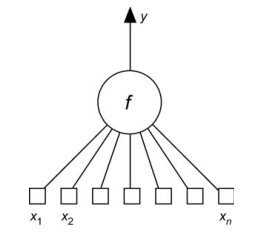
\includegraphics[width=0.5\textwidth]{media/literature/artificial-neuron1.png}
        \rule{35em}{0.5pt}
        \caption[Example of an artifcial neuron]{\textbf{Artificial Neuron} -- a nonlinear bounded function $y = f(x_{1}, x_{2},\ldots,x_{n};w_{2},\ldots,w_{n})$ where the ${x_{i}}$ are the input values and the  ${w_{i}}$ are the weights of the neuron~\citep{Dreyfus2005}.}\label{fig:an}
\end{figure}


A weight is assigned to each of a neuron's inputs. They are the coefficients of a neuron's equation and therefore reflect the importance of individual inputs. A bias is a constant value assigned to each neuron. They are used to shift a neuron's activation function output in a positive or negative direction~\citep{Malik2019weights}.

A \Gls{nn} is made up of a series of layers; an input layer,
a number of hidden layers, and an output layer. Each layer is
made up of a set of neurons, where each neuron is fully connected
to all neurons in the previous layer. Each neuron within a single layer
does not share connections with, and operates completely independently from one another~\citep{cs231n}.


Using the case of \Gls{cv} as an example, 
the input layer of a \Gls{nn} consists of
neurons encoding the values of image pixels (RGB or greyscale intensities).
The encoding is typically achieved by passing the raw input 
value through an activation function which outputs a normalised value. 
Often, activation functions in modern \Glspl{nn} output non-linearities, 
an example is to use a Sigmoid Function which maps an input to a value between 0 and 1 
(\textit{see Fig.~\ref{fig:activation} \textit{left}})~\citep{Nielsen2015}.

However a more common activation function found in current \gls{nn} models is the \gls{relu}.
Although computed as a piecewise linear function, \gls{relu} also adds non-linearity to the output. The \gls{relu} function maps an input to a value
within the range of $0 \text{ and } \infty$ (\textit{see Fig.~\ref{fig:activation} \textit{right}})~\citep{Malik2019activation}.

\begin{figure}[H]
    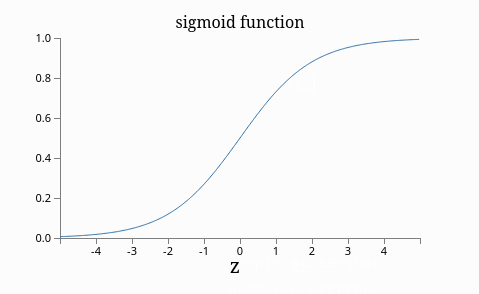
\includegraphics[width=0.5\textwidth]{media/literature/sigmoid.png}
    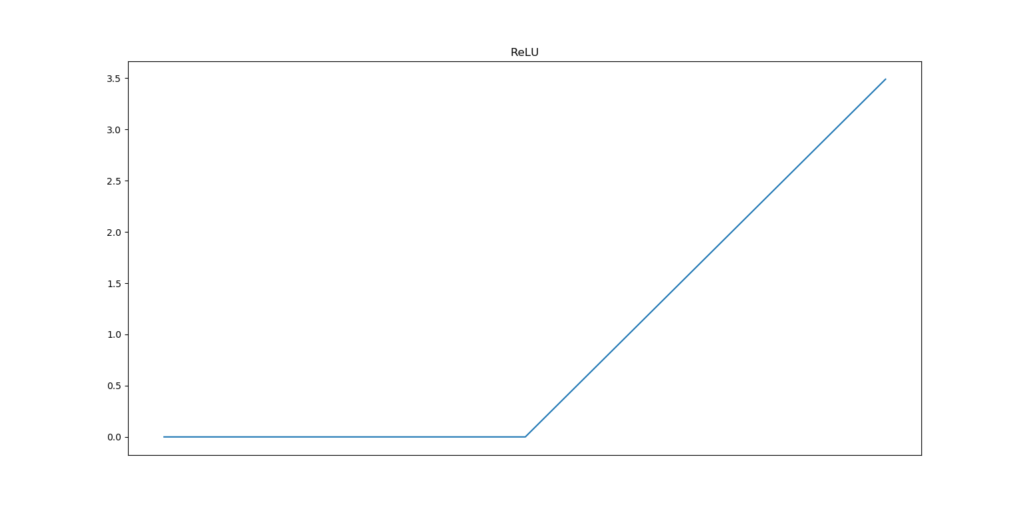
\includegraphics[width=0.5\textwidth]{media/literature/relu.png}
    \rule{35em}{0.5pt}
    \caption[Examples of activation functions]{\textit{Left}: The Sigmoid Function is one type of activation function. `A bounded, differentiable, real function that is defined for all real input values and has a non negative derivative at each point'~\citep{Han1995}. \textit{Right}: An example of a \Gls{relu} activation function transforming $x$ to a value between $0 \text{ and } \infty$~\citep{Malik2019activation}.}\label{fig:activation}
\end{figure}


The output layer of a \gls{cv} classification network contains neurons representing the class
scores of the task (\textit{see Fig.~\ref{fig:nn}}). For example, in a \gls{nn} attempting to classify handwritten
digits, the output layer would contain 10 neurons, representing the digits 0 - 9.
If the first neuron fires, i.e.\ has an output $\approx 1,$ this will indicate that the
network is confident the handwritten digit is 0, and so on~\citep{Nielsen2015}.

\begin{figure}[H]
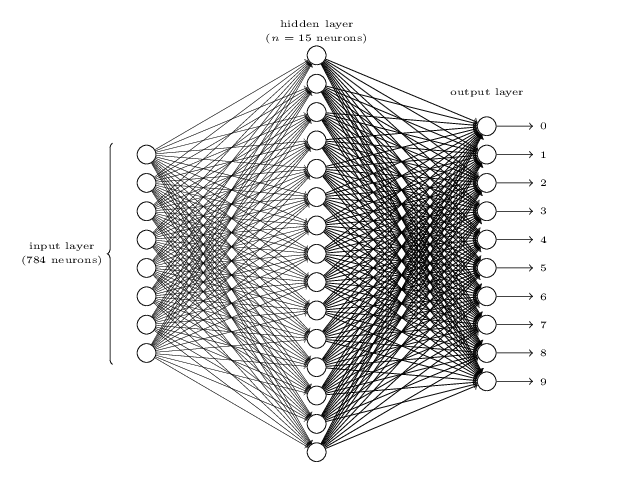
\includegraphics[width=1\textwidth]{media/literature/handwrittenDigitNN.png}
    \rule{35em}{0.5pt}
\caption[Example of a neural network]{Neural Network. Example of a \Gls{nn} to
classify handwritten digits. The input is a single vector of 28x28 pixels, i.e. 784 neurons, and outputs
10 neurons representing digits 0-9~\citep{Nielsen2015}.}\label{fig:nn}
\end{figure}

% TODO: explain what deep learning is in context of  nns
\glspl{nn} with a single hidden layer are able to approximate functions that contain any 
continuous mapping from one finite space to another, whereas with no hidden layers a \gls{nn}
model would only be able to represent linear functions or decision boundaries~\citep{hornik1991}.

\begin{figure}[H]
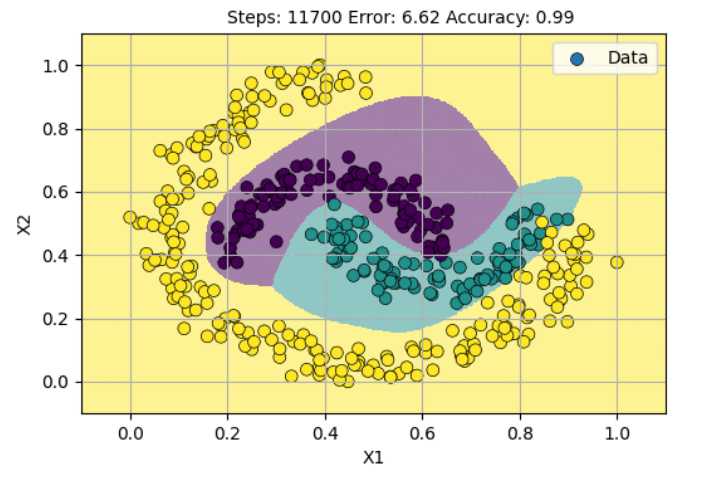
\includegraphics[width=1\textwidth]{media/literature/deep-boundary.png}
    \rule{35em}{0.5pt}
    \caption[Complex decision boundary from deep neural network]{\textbf{Complex Decision Boundary} -- Example of a decision boundary made capable by deep learning~\citep{sapkota2020}}\label{fig:dnn-decision}
\end{figure}

\glspl{nn} are especially powerful when additional hidden layers are
added to a network's architecture. By doing so, a model can not only approximate continuous functions
to a high accuracy with less computational cost, but it can also represent complex composite 
functions~\citep{sapkota2020}. An example of the complex decision boundaries that are possible from
\glspl{nn} with more than one hidden layer can be seen in \textit{Fig.~\ref{fig:dnn-decision}}.

\glspl{nn} with two or more hidden layers fall under the category of deep learning, and are often referred to as
\Glspl{dnn} or \Glspl{mlp}. This subset
of \gls{ml} has become increasingly powerful with the rise of powerful variations of \glspl{dnn}, namely \Glspl{cnn} and \Glspl{rnn} in recent years
due to their successes within the field of \gls{cv}.
% TODO make this paragraph nicer (add refs etc)

\subsection{Gradient Descent \& Backpropagation}
% TODO: explain how nns can be trained using backpropagation
Training a \gls{nn} consists of iteratively adjusting the values of weights at
each neuron in order to minimise the model's output error. Although there
are many algorithms available for determining the optimum values of weights, a common approach
is to use some flavour of \textit{gradient descent} 
together with a technique for efficiently computing partial derivatives within a directed graph called \textit{backpropagation}.

There are three main variants of gradient descent; vanilla gradient descent or \Gls{bgd}, \Gls{sgd}, and \Gls{mbgd}.

\gls{bgd} computes the gradients of a cost function with regards to the weights within an entire training set.
The cost function can take many forms depending on the architecture of the \gls{nn} and the task it is concerned with,
however the main principle behind it is to map the different
values of each weight to a score which determines how well the model performs~\citep{shung2018}.

\begin{figure}[H]
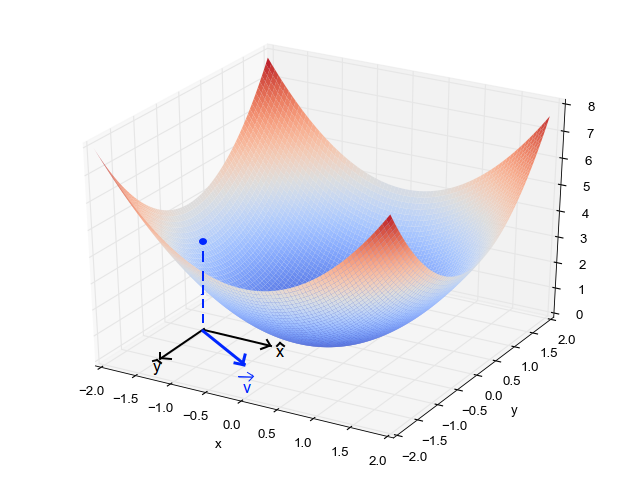
\includegraphics[width=1\textwidth]{media/literature/gd-example.png}
    \rule{35em}{0.5pt}
    \caption[Example visualisation of gradient descent]{\textbf{Visualisation of Gradient Descent Search Space} -- An example of an \textit{ideal} search space, where the vertical $z$ axis shows the cost function $f(x, y)$, and $\vec{v}$ represents the resulting direction of the maximum gradient applied to the parameter in question~\citep{bendersky2016}.}\label{fig:gd-example}
\end{figure}

A search space can then be defined by plotting the output of a cost function against the values of the weights
it is concerned with, an example of such a search space with two weights can be seen in \textit{Fig.~\ref{fig:gd-example}}.
As the number of weights increases, the harder it becomes to visualise the contours of a multi-dimensional plane. 
\gls{bgd} then computes the directional derivative of this plane given a set of weight values, and uses this value
as a vector with a magnitude defined by a \textit{learning rate} hyper-parameter to update the weights of the network~\citep{ruder2017}.

\gls{sgd} attempts to reduce the number of 
computations during training by only performing updates
to weights for each training example instead of recomputing gradients for similar weights
at each iteration. By removing these redundant calculations, \gls{sgd} typically decreases the time taken
to converge to an optimum solution of weights. Additionally, due to the high variance of
each update, and so long as the learning rate is steadily decreased at each iteration, \gls{sgd} has an equal
chance at finding the global minimum to \gls{bgd}~\citep{ruder2017}.

\gls{mbgd} on the other hand, attempts to combine the benefits from \gls{bgd} and \gls{sgd} by 
performing an update for every mini-batch of $n$ training examples. Therefore, allowing for the precision of
\gls{bgd} with similar speeds as \gls{sgd}.

Backpropagation is a computational technique commonly used within \gls{nn} training for calculating
partial derivatives used for gradient descent algorithms in linear time with respect 
to the number of weights being optimised. This is an important
step in order to train \glspl{nn} within a sensible timeframe, considering the potentially
high volume of weights that are needed for complex tasks. A more detailed 
investigation into this technique will be discussed later in this chapter (\textit{Section~\ref{section:paradigms}}).

\subsection{Vulnerabilities to Adversarial Attacks}\label{section:adversarial}

\glspl{nn} and \glspl{dnn} have been adopted and deployed within a wide
range of industry applications for tasks such as speech recognition or facial recognition, 
and have shown to perform adequately for many of these tasks. However, as mentioned in \textit{Chapter~\ref{Chapter1}}, \glspl{nn} have been shown to be
vulnerable to adversarial attacks. Specifically, by adding small, imperceptable changes
to the input features, can lead to abnormal behaviours such as missclassification in the output layer.

% 3 examples of adversarial attacks on nns (not Google's sticker one)
This observation was first made in 2014,
which found properties of \glspl{nn} that cause them to learn uninterpretable solutions that could have counter-intuitive properties when
imperceptable non-random pertubartions are made to a test input, known as \textit{adversarial examples}~\citep{szegedy2014}. 
Interestingly, these examples were shown to be robust, such that they have the same effect
across models with varying architectures, activation functions, or trained on different data sets altogether. A tentative
explanation for this phenomenon was to blame the non-linear nature of \glspl{nn}, and cases of poor generalisation on test data.

\begin{figure}[H]
\center
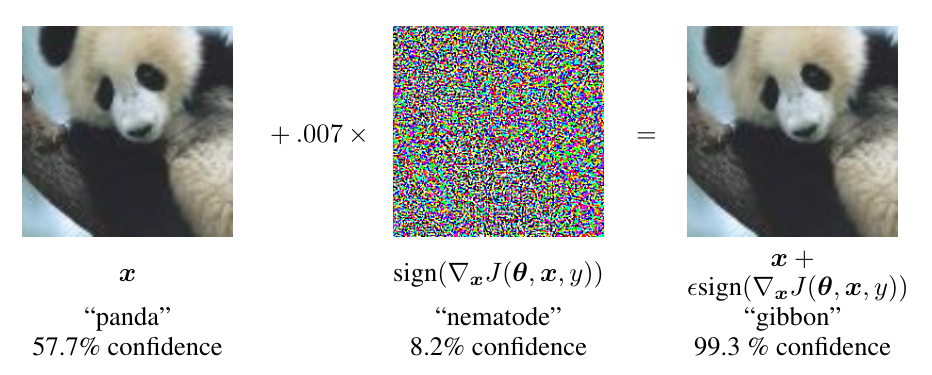
\includegraphics[width=0.9\textwidth]{media/literature/adversarial-example.png}
    \rule{35em}{0.5pt}
    \caption[Demonstration of the effects of adversarial examples]{\textbf{Effects of Adversarial Examples} -- A demonstration of the effects of adversarial examples; an input image of a panda with added noise causes the model to missclassify the image as a gibbon~\citep{goodfellow2015}.}\label{fig:adversarial-example}
\end{figure}

However in 2015, further attempts to explain \gls{nn} vulnerabilities to adversarial examples argued
that it was not the non-linear nature, but rather the linear behaviour of \glspl{nn} which is sufficient 
to cause adversarial examples~\citep{goodfellow2015}. This claim was supported by the authors' demonstration that
leveraging non-linear \gls{nn} families such as \Glspl{rbfn} can significantly reduce the vulnerabilities to adversarial examples.

\begin{figure}[H]
\center
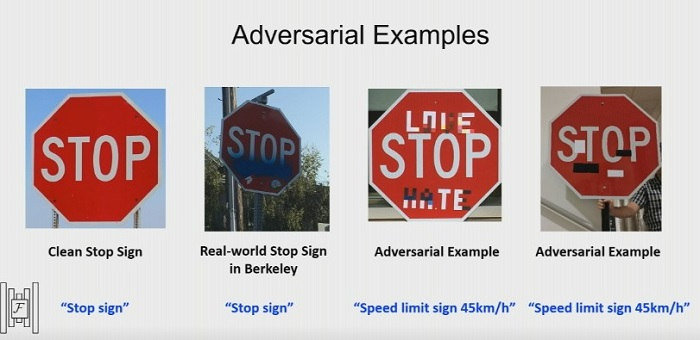
\includegraphics[width=0.9\textwidth]{media/literature/stop-sign.jpg}
    \rule{35em}{0.5pt}
    \caption[Demonstration of the effects of adversarial examples in real world]{\textbf{Effects of Adversarial Examples in Real World} -- A demonstration of how adversarial examples can be used in real world situations to cause misclassification of stop signs~\citep{eykholt2018}.}\label{fig:stop-sign}
\end{figure}

Research in 2018 showed that adversarial examples can be 
used in real world situations in order to fool a \gls{dnn} used for street sign 
recognition within a self-driving car's navigation system by placing black and white stickers
on street signs (\textit{see Fig.~\ref{fig:stop-sign}})~\citep{eykholt2018}.

These vulnerabilities have demonstrated that \gls{nn} technology has yet to reach the level of
maturity necessary for applications in safety-critical systems, and have raised
concerns over the robustness of \glspl{nn} in general.


\subsection{Descrimination \& Neural Networks}\label{section:descrimination}

Aside from vulnerabilities caused by intrinsic properties of \glspl{nn}, there are
issues which stem from the data being used to train supervised models too. That is,
if the training data has inherent bias towards or against a specific class within the domain, the output 
of the model trained on that data will reflect these biases (\textit{see Fig.~\ref{fig:bias-nn}}). 
Subsequently, when bias data is used to train \glspl{nn} used in applications which have either a direct or
indirect affect on people's lives, there is a chance that they can result in simulated descrimination of certain social groups.

\begin{figure}[H]
\center
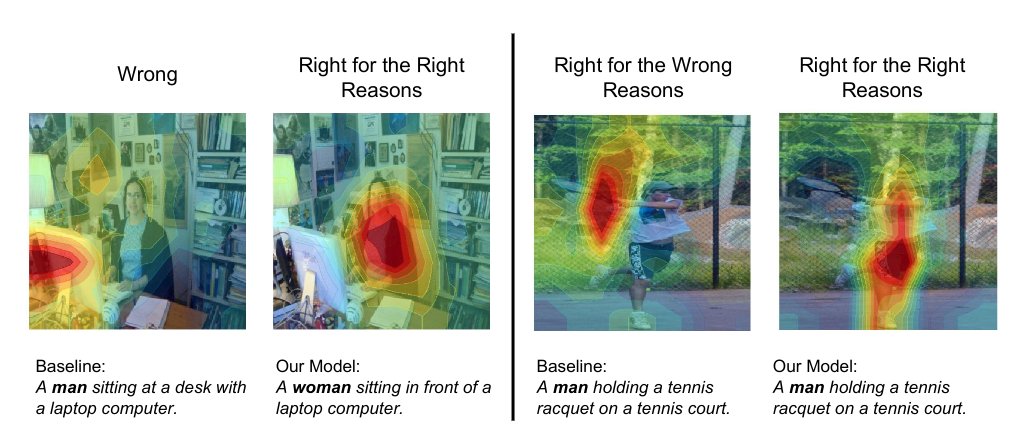
\includegraphics[width=1\textwidth]{media/literature/bias-nn.png}
    \rule{35em}{0.5pt}
    \caption[Example of negative bias effects in neural networks]{\textbf{Discriminating Bias in Training Data} -- An example of how image captioning \glspl{nn} use the features present in a bias data set to generate either incorrect captions (\textit{left}), or use the wrong features to generate correct captions (\textit{right})~\citep{burns2019}.}\label{fig:bias-nn}
\end{figure}

In recent years, there have been many attempts to mitigate the effects of unwanted bias in 
data being fed to \glspl{nn}. These include work in facial recognition, where a model is trained
separately on demographic representations prior to being trained on face attribute data, thus 
preserving potential users' demographic privacy~\citep{ryu2018}; or more recently, developing new regularisation techniques for \Glspl{gan} which 
allow a model to categorise classes while ignoring bias features in the training data~\citep{kim2019}.


Although there has been significant progress in this area of research and that discussed in \textit{Section~\ref{section:adversarial}}, 
many of the proposed solutions
have not yet become ubiquitous in industry. As such, there
is a need for creating formal methods which allow developers to verify the fairness and robustness of their
systems in a wide range of programming environments.
%----------------------------------------------------------------------------------------
%	SECTION Formal Verification
%----------------------------------------------------------------------------------------

\section{Formal Verification}

Formal verification is a mature and extensive discipline which has seen development in many areas 
of software engineering. As such, this section will attempt to provide a succinct 
overview of the ideas behind formal verification while keeping the focus on areas
related to this thesis.

\subsection{Background}

Although formal verification stems from a long history of development within the fields
of classical and first-order logic~\citep{smith2011, boole2009, russell1937}, this thesis is concerned with modern formal methods
used for software engineering tasks, and thus will use the following definition.

Formal verification is defined by a set
of mathematical tools used to analyse the space of possible system 
states both in hardware and software~\citep{seligman2015}. In other words,
checking that a system will not produce abnormal behaviours given a 
specific input, or to verify the correctness of hardware or software design~\citep{grout2008}.

Early software systems were typically verified by hand when necessary. However, as 
the size and complexity of software increased over time, so too did the computational
cost of exhaustively verifying them. As such, huge efforts have been made over the past few decades
to develop formal methods frameworks which utilise the power of computing for software engineers.

\subsection{Theorem Provers}

The earliest approach for formally verifying software, and still commonly used, is with theorem provers.
Theorem provers were initially developed as interactive, or computer assisted frameworks, however over
time the much harder task of automated theorem provers were introduced.

These tools allow developers to formalise theorems using some variant of mathematical logic,
such as propositional logic, predicate logic, or first-order logic to name a few. Then, by 
using \textit{proof checking}, one can establishes the validity of a theorem by mechanically checking the proof~\citep{geuvers2009}.


\subsection{Model Checkers}

Model checking is another branch of formal verification for software that
came along after theorem provers. This technique consists of three main tasks, \textit{modelling}, \textit{specification}, and \textit{verification}.

Modelling is the process of converting a system design into a formalism accepted by a model checking tool. Once this process has 
finished, a specification of the properties in which a design should satisfy must be provided before verification. Once a model and
a specification have been provided, the process of verifying the system can occur. In an ideal world, the final stage can be automated, but
often it is necessary to manually analyse the verification results~\citep{clarke2018}.

In other words, given a program $P$ and a specified property $\phi$, the primary goal of a model checker
is to search the space of possible states of $P$, and ensure that $\phi$ holds in all scenarios~\citep{zhang2019}.
%----------------------------------------------------------------------------------------
%	SECTION Formal Verification AI
%----------------------------------------------------------------------------------------

\section{Formal Verification of Neural Networks}

In recent years, there has been growing interest in using formal verification tools
within the field of \gls{ai}~\citep{russell2016}. Although there have been promising advancements
in areas such as \gls{mas}~\citep{lomuscio2017, kouvaros2016}, there is significantly less research
regarding the formal verification of \glspl{nn}.

The most common methods for evaluating \glspl{nn} rely on testing models on 
previously unseen data, which can provide statistical guarantees regarding accuracy
and generalisation. However this approach tends to be incomplete as it does not provide an 
exhaustive search of all possible inputs to the network~\citep{akintunde2020}.

Initial attempts at formally verifying \glspl{nn} focused on using \textit{reachability }\textit{analysis }as 
a verifiable property. \textit{Reachability }\textit{analysis} is concerned with determining whether
a given state is reachable in a number of steps from an initial state of a system \citep{akintunde2018}.
The idea behind conducting such an analysis, is that it is then possible to verify
that an unwanted state of a system such as those discussed in \textit{Sections~\ref{section:adversarial} \&~\ref{section:descrimination}} 
is never reached during the lifecycle of the system.

% katz


% sappire

Thus far, this area of research is still in its early stages, however fast progress has been made
in demonstrating how it is possible to achieve real-world scalability \textit{w.r.t }verifying \glspl{nn}~\citep{pulina2010, xiang2018}, including 
a handful of deep structures such as \glspl{cnn}~\citep{kouvaros2018} and \glspl{rnn}~\citep{zhang2020}.

Additionally, progress has been made in developing tools designed to utilise the many formal methods that
have been worked on for decades which allow developers to analyse and verify their models easily.
This includes tools such as the Maribou Framework for \glspl{dnn}~\citep{katz2019}, which builds on the 
authors' previous work in using \gls{smt}-based techniques to verify \glspl{dnn}; and
the Sapphire Python library~\citep{kokke2020}, which translates TensorFlow feed-forward \gls{nn} model queries to the Z3 \Gls{smt} solver created by Microsoft Research~\citep{demoura2008}.

However, as \gls{nn} development is starting to become prevalent across a wider range of programming languages and
paradigms, it is important for further work to be made in developing new frameworks for formally verifying \glspl{nn}, and to 
investigate how different programming language infrastructures can affect this development.

%----------------------------------------------------------------------------------------
%	SECTION PROGRAMMING PARADIGMS FOR ML
%----------------------------------------------------------------------------------------
\section{Programming Paradigms for Deep Learning}\label{section:paradigms}

As \glspl{nn} and \glspl{dnn} become more and more ubiquitous in software applications, so to does
the number of weights needed for them to perform adequately for their tasks. As such, an enormous amount
of work has gone into ensuring the toolkits used by \gls{ml} engineers allow for scalable and efficient development
of such models.

\subsection{Auto Differentiability}

\subsection{Computational Graphs}

%----------------------------------------------------------------------------------------
%	SECTION PROGRAMMING The Go Programming Language
%----------------------------------------------------------------------------------------
\section{The Go Programming Language}

\subsection{Brief History}
\subsection{Go for ML}
\subsection{Go for Formal Verification}

%----------------------------------------------------------------------------------------
%	SECTION CONCLUSIONS
%----------------------------------------------------------------------------------------
\section{Conclusions}

%\input{Chapters/Chapter2} 
%\input{Chapters/Chapter3}
%\input{Chapters/Chapter4} 
%\input{Chapters/Chapter5} 
%\input{Chapters/Chapter6} 
%\input{Chapters/Chapter7} 

%----------------------------------------------------------------------------------------
%	THESIS CONTENT - APPENDICES
%----------------------------------------------------------------------------------------

\addtocontents{toc}{\vspace{2em}} % Add a gap in the Contents, for aesthetics

\appendix % Cue to tell LaTeX that the following 'chapters' are Appendices

% Include the appendices of the thesis as separate files from the Appendices folder
% Uncomment the lines as you write the Appendices

% Appendix A

\chapter{Appendix Title Here} % Main appendix title

\label{AppendixA} % For referencing this appendix elsewhere, use \ref{AppendixA}

\lhead{Appendix A. \emph{Appendix Title Here}} % This is for the header on each page - perhaps a shortened title

Write your Appendix content here.
%\input{Appendices/AppendixB}
%\input{Appendices/AppendixC}

\addtocontents{toc}{\vspace{2em}} % Add a gap in the Contents, for aesthetics

\backmatter

%----------------------------------------------------------------------------------------
%	BIBLIOGRAPHY
%----------------------------------------------------------------------------------------

\label{Bibliography}

\lhead{\emph{Bibliography}} % Change the page header to say "Bibliography"

\bibliographystyle{apalike} % Use the "apalike" BibTeX style for formatting the Bibliography

\bibliography{Bibliography} % The references (bibliography) information are stored in the file named "Bibliography.bib"

\end{document}
